\documentclass[../../relatorio.tex]{subfiles}
\begin{document}
Utilizando a estrutura apresentada no Diagrama de Componentes (ver \ref{sec:diagrama_componentes}),
desenvolveu-se vários Diagramas de Classe para representar as classes que compõe cada um dos sistemas.
Atendendo que o sistema com maior complexidade é o \textit{ReparacoesLN}, foi neste que o grupo se debruçou
mais afincadamente. Utilizou-se uma estratégia \textit{\textbf{Facade}} a estrutura desta classe.

Como já referido, através da análise dos casos de uso, identificou-se um conjunto
de métodos necessários para a sua implementação.
Estes métodos foram colocados ao nível da API \textit{IReparacoesLN}.
Posteriormente, implementou-se a interface através da classe \textit{ReparacoesLNFacade}.
Sendo este o ponto de entrada na camada de negócio, deve conhecer cada um dos subsistemas necessários.
Assim, criou-se uma variável de instância para cada uma das API dos subsistemas:
\textit{IGestClientes} (ver \ref{sec:ss_clientes}), \textit{IGestReparacoes} (ver \ref{sec:ss_reparacoes}) e
\textit{IGestColaboradores} (ver \ref{sec:ss_colaboradores}).
Desta forma, passa a ser possível utilizar a estratégia de \textit{\textbf{Facade}} para realizar a implementação
dos casos de uso propostos, i.e. tem-se uma classe agregadora que permite um ponto de entrada na camada da lógica.

Para a construção das classes necessárias para suportar as funcionalidades requisitadas,
começou por se analisar o Modelo de Domínio (\ref{modelacao_dominio}) e converter as entidades
em classes.
Após uma fase inicial, para além de se ter verificado que a modelação de domínio realizada
na fase I não era suficiente, foi, ainda, necessário criar algumas \textbf{classes de implementação}
para melhorar a eficiência e facilitar a implementação, tais como \textit{Precos}, \textit{CustoTotalReparacao},
\textit{ReparacoesPorMes} e \textit{GestAgenda}.
Estas classes serão abordadas nos respetivos sistemas.

\begin{landscape}
    \begin{figure}[!ht]
        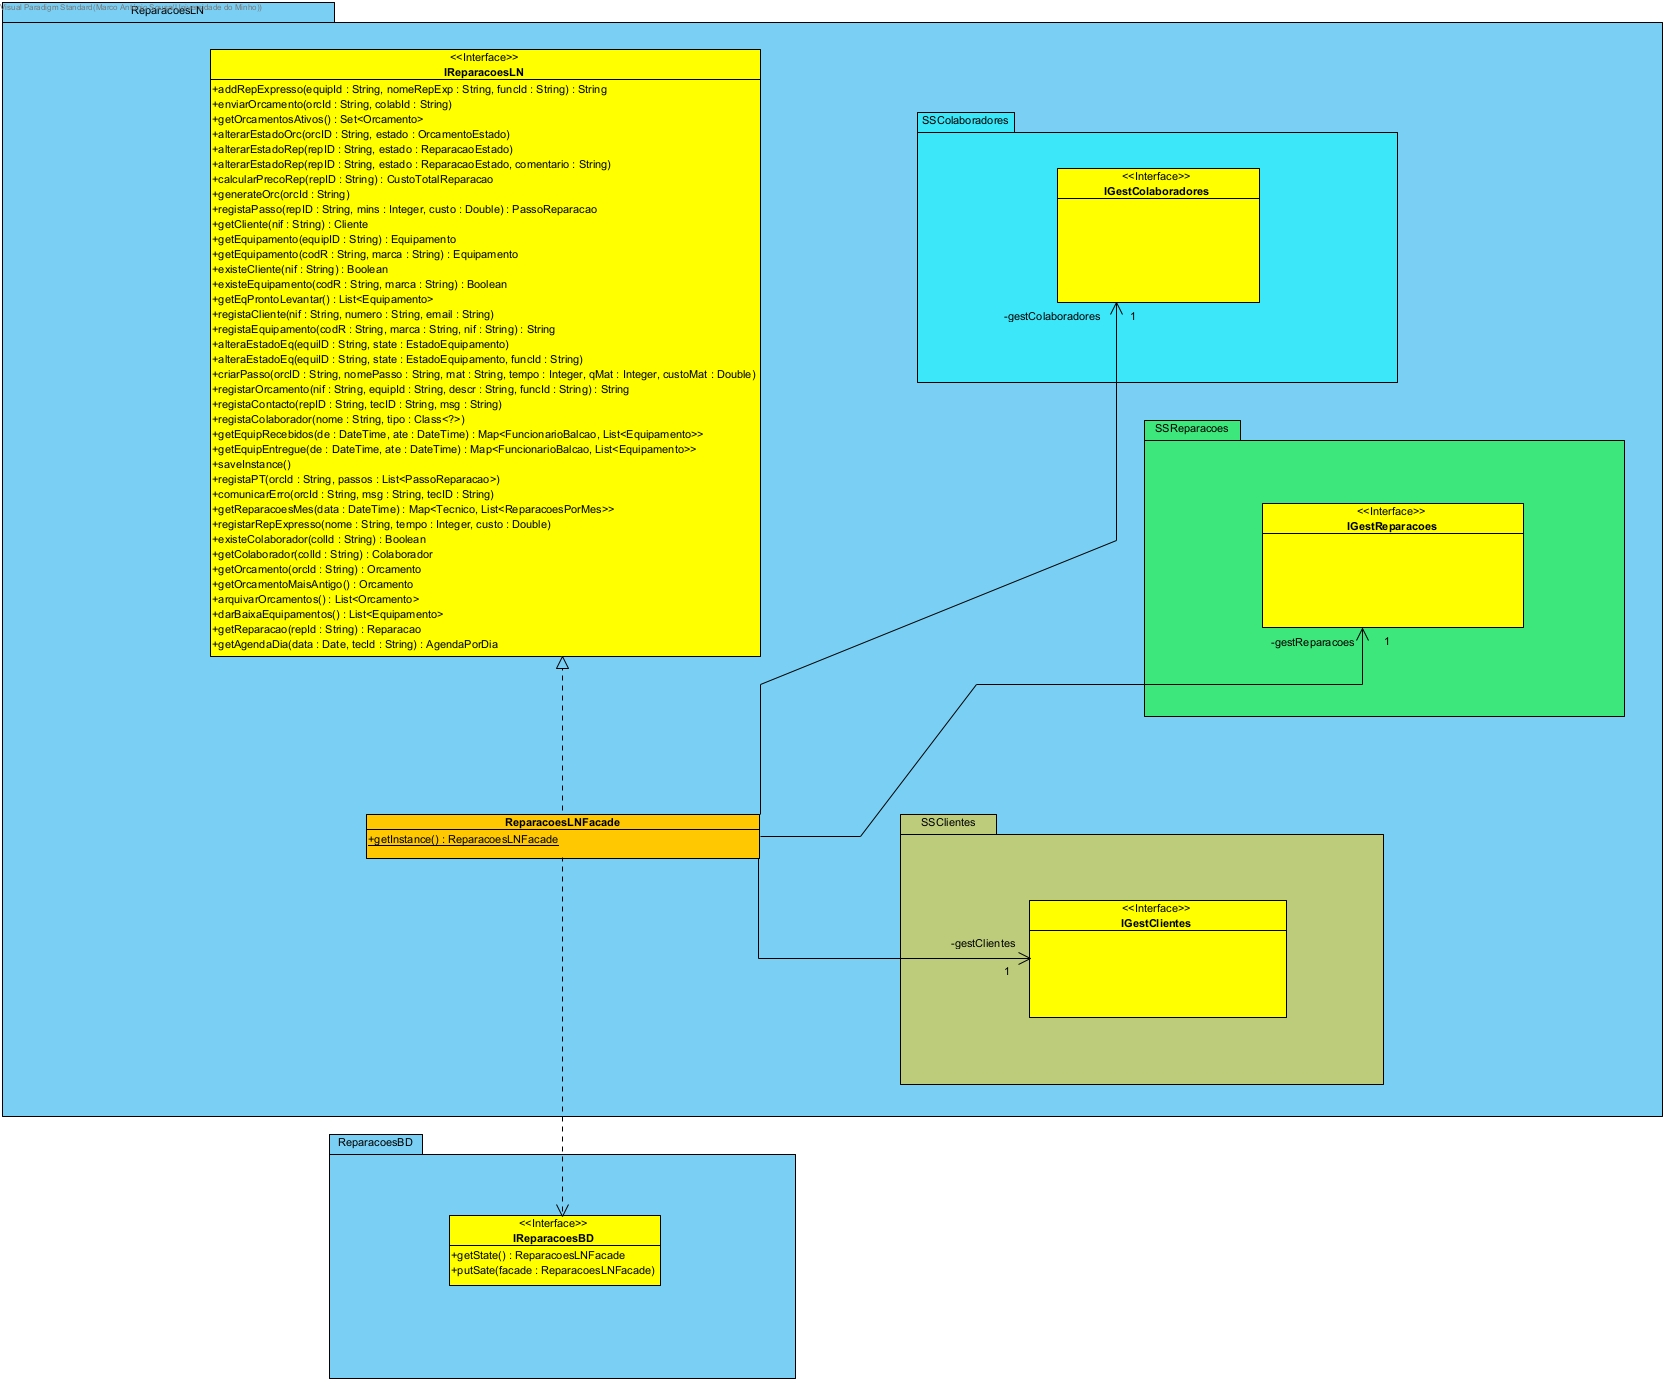
\includegraphics[scale=0.3]{ReparacoesLN.jpg}
        \caption{Diagrama de Classe - ReparacoesLN}
    \end{figure}
\end{landscape}

\subsubsection{SS Clientes} \label{sec:ss_clientes}
\subfile{model_funcional/classe/ss_clientes.tex}

\subsubsection{SS Colaboradores} \label{sec:ss_colaboradores}
\subfile{model_funcional/classe/ss_colaboradores.tex}

\subsubsection{SS Reparações} \label{sec:ss_reparacoes}
\subfile{model_funcional/classe/ss_reparacoes.tex}

\subsubsection{Classes de Implementação} \label{sec:classes_implementacao}
\subfile{model_funcional/classe/classes_implementacao.tex}

\end{document}